\section{Approach}

Given that compute performance was a key objective in this project, we adopted a middle-out\cite{middleout} design strategy by building tools and interfaces around those tools that enhance capability while introducing minimal system overhead. Middle-out design is more complex and requires maturity of knowledge pertaining to the existing system, but allows for deep restructuring without the overhead of a ground-up redesign. 

%% Team Organization
\subsection{\cancel{Team} Project Organization}
We strongly felt that middle-out design was the optimal approach due to inter-dependencies between several sub-components. For example, while it would be beneficial to implement a highly optimized matrix-multiply operation, those performance improvements would not translate to other algorithms. In general, improving LCDK performance across the board would mean countless hours of tinkering with a multitude of algorithms, each with it's own unique degree of optimizability. Alternatively, one could heavily optimize only matrix-multiply and then successfully (and approximately!) transform most problems into their matrix-multiply analogs, which is what we did with neural networks (later we will show that neural networks are Turing complete). In general our strategy was to transform problem-sets into neural-network analogs, and process them in real-time using the feed-forward step on our matrix-multiply optimized neural network.

%% Standard (de jure, e.g., 802.11n; and de facto, e.g., tools commonly used, such as FFT, Melfrequency):
\subsection{Standard}
A core component of this project included implementing de jure standards such as I\textsuperscript{2}C, UART and GPIO communication protocols. Other components required the implementation of well-known methodologies such as feed-forward step in a multilayer-perceptron, or de facto standards such as neuron activation functions in a neural network (tanh, reLU, sigmoid).

%% Theory:
\subsection{Theory}

\subsubsection{Compute Performance}
For a given operation, we measure compute performance of as a function of system resources consumed - such as memory, CPU clock-cycles elapsed, and bus usage. Together, these factors contribute to overall system throughput and latency. In order to effectively improve latency, we intend to record and benchmark lower level metrics such as memory and clock cycles for a series of publicly available libraries. These include TI provided assembly implementations of DSPLIB and MATHLIB, along with math.h from the GNU compiler.\\

\subsubsection{Communication Protocols} Theoretical basis for the I\textsuperscript{2}C, UART and GPIO protocols are discussed below.\\\\
\textbf{The I\textsuperscript{2}C Protocol}\\
The Inter-integrated Circuit (I\textsuperscript{2}C) Protocol\cite{i2c} is an asynchronous protocol that allows multiple slave devices to communicate with multiple master devices on the same bus. Operating in either 100kHz or 400kHz mode, the LCDK exposes two independent I\textsuperscript{2}C buses, multiplexed with SPI on the J15 connector header. I\textsuperscript{2}C is a intra-bus connection protocol, therefore enabling long distance communication requires the addition of bus-buffers that circumvent the issue of bus capacitance.
\begin{figure}[h!]
  \caption{I\textsuperscript{2}C Addressing and Message Frame}
  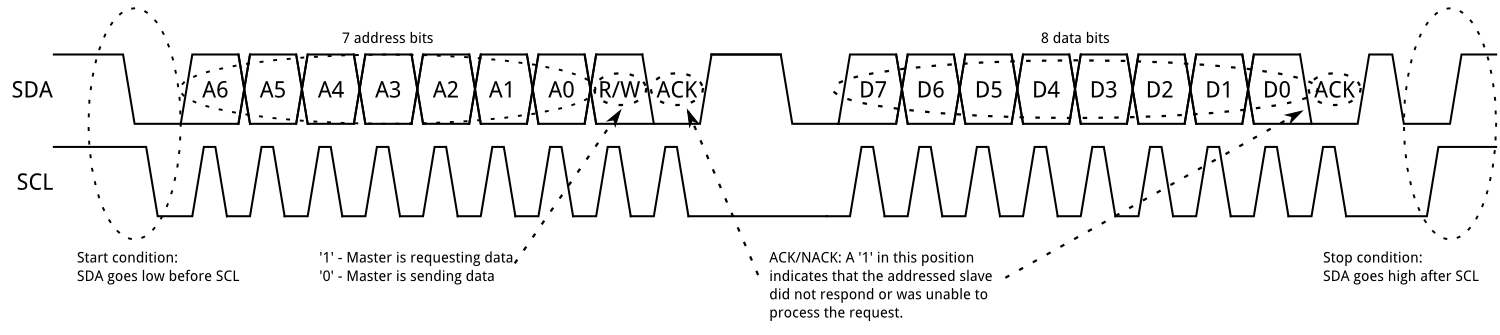
\includegraphics[width=0.5\textwidth]{images/i2c_protocol.png}
\end{figure}
I\textsuperscript{2}C messages comprise two types of frames, namely an address frame and a message frame. Together, these frames provide the receiver all the information it needs to store the incoming byte into the requested location. Data is sent over the SDA channel once SCL has been set to low, and it polled again after SCL is set to high. The address frame is always sent first. I\textsuperscript{2}C implements 7-bit and 10-bit addressing. 

\textbf{The UART Protocol} \\
Universal Asynchronous Receiver/Transmitter (UART) is a data format and transmission speed configurable serial data transfer protocol. Data is transmitted bit-wise and reassembled at the destination into a complete word. After the transmission of a complete word, a stop bit it sent to the receiver. The data frame in the figure below illustrates this implementation.
\begin{figure}[h!]
  \caption{UART Data Frame}
  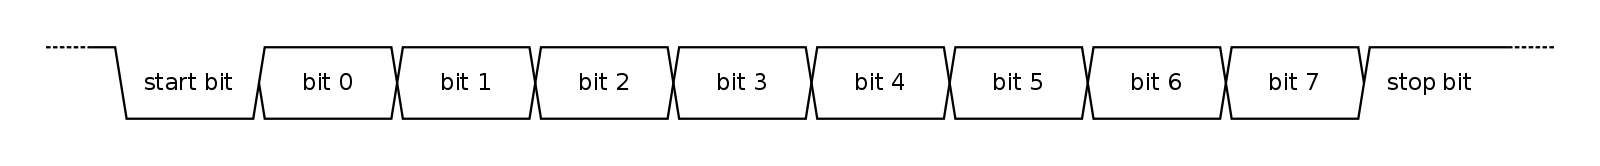
\includegraphics[width=0.5\textwidth]{images/uart.png}
\end{figure}

\textbf{GPIO}\\
By definition, General-purpose input/output (GPIO) implements a generic protocol-less interface, with ability read or write HIGH/LOW voltages to a given set of pins. In this way, they are a building block for higher-level protocols. The ability to be able to demonstrate fine-control of these pins indicates the potential capability of being able to implement low-bandwidth interfaces of any of type. Although GPIO is quite flexible, it is fully CPU bound, since every event on the bus that generates an interrupt has to be handled by the CPU immediately.\\

\subsubsection{Deep Neural Network}
The \textbf{Universal Approximation Theorem}\cite{ufa} for artificial neural networks states "A feed-forward network with a single hidden layer containing a finite number of neurons can approximate continuous functions on compact subsets of R\textsuperscript{n}, under mild assumptions on the activation function". This indicates that neural networks can represent a wide variety of interesting functions for well chosen weight-parameters. We leverage this powerful capability to transform complex DSP algorithms into weight matrices for neural networks and implement these networks using efficient matrix multiplication operations.

%% Software/Hardware %% Operation (how your system works):
\subsection{Operation - Software/Hardware}

\subsubsection{Compute Performance}
Included in the file profiler.h are timing functions that count clock-ticks, and as such can be used for creating small and effective benchmarks (with clock-cycle level accuracy) when profiling LCDK code. Cycle count is independent of clock frequency and therefore a better metric for work-done than elapsed time. This functionality is implemented by keeping track of the clock registers on the processor and plays a pivotal role in bench-marking/profiling code. Effective use of external libraries such as DSPLIB, MATHLIB, and IMGLIB (all of which provide assembly-optimized implementations of commonly used DSP and math functions) mandates precise and accurate bench-marking, which can be achieved using this library.\\

\subsubsection{Communication Protocols}
In this section, we will omit the overview for UART and GPIO since the theory covers the principle of operation, and the procedure covers the concrete implementation.\\
\textbf{I\textsuperscript{2}C with 9-DOF MPU-9250}
\begin{figure}[h!]
  \caption{MPU-9250 System Overview}
  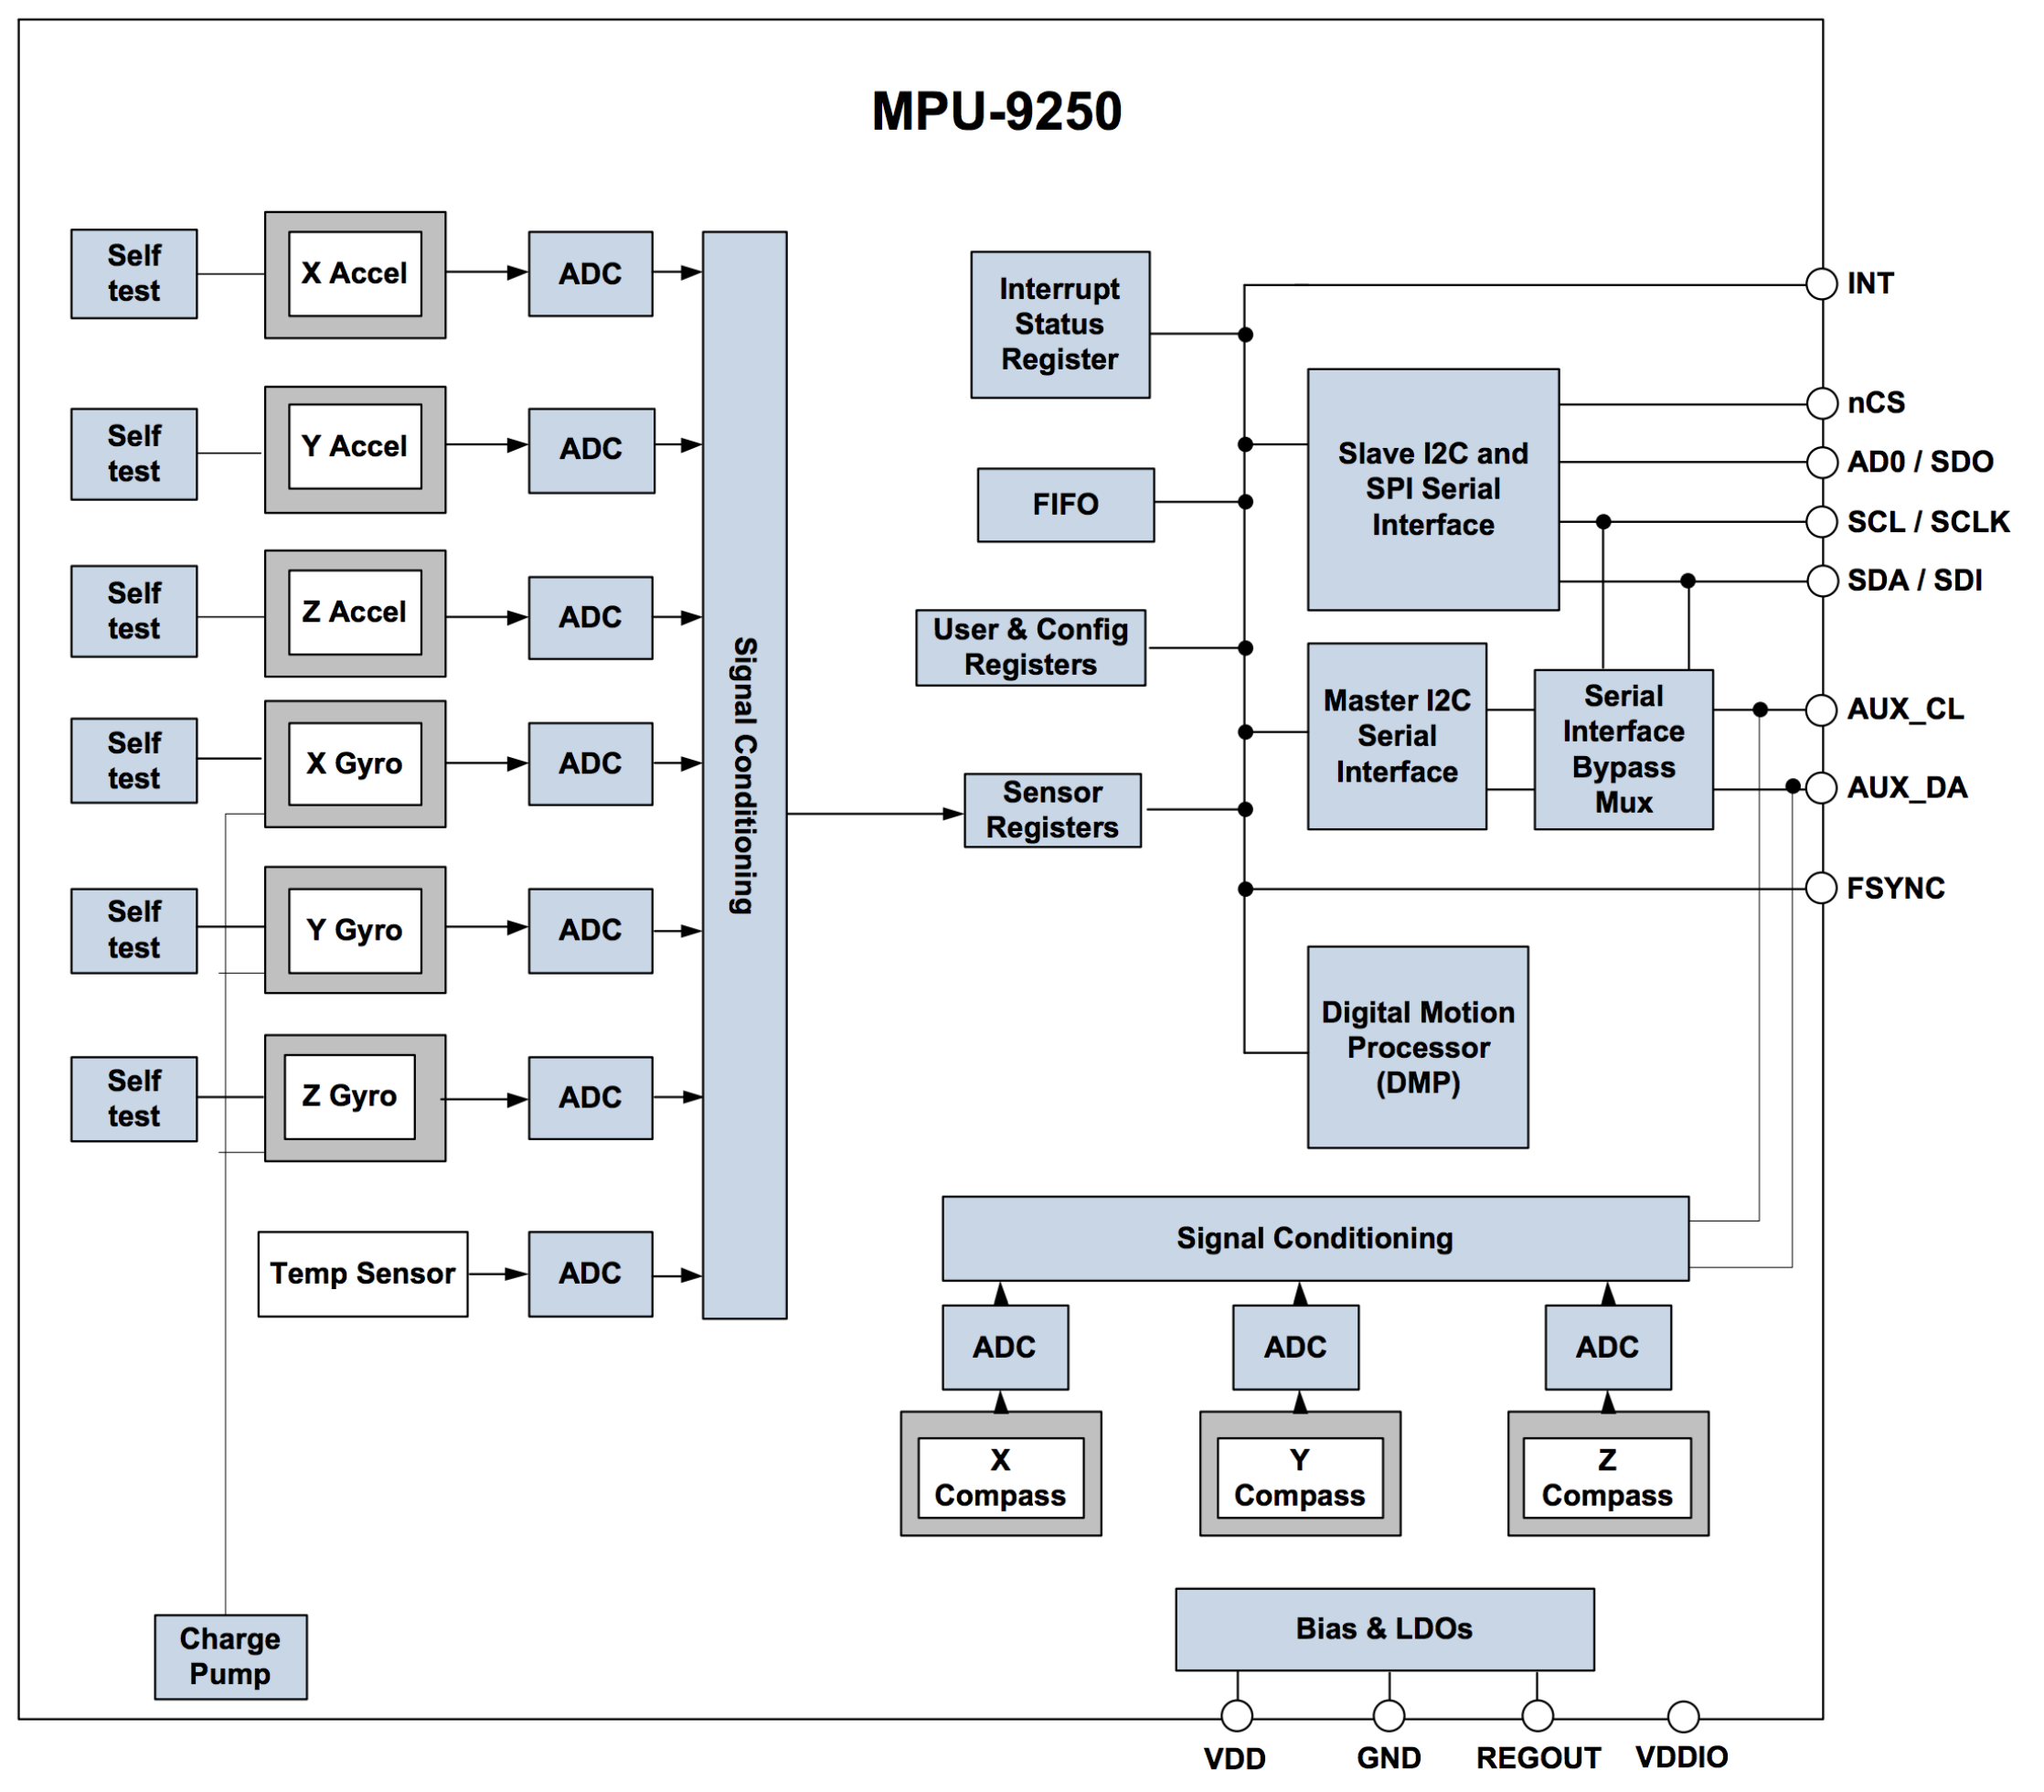
\includegraphics[width=0.5\textwidth]{images/9250.png}
\end{figure}
Next, we will interface the InvenSense MPU-9250 9-DOF with the LCDK over I\textsuperscript{2}C. The figure above illustrates the system diagram for the MPU-9250. The 9250 chipset is a fairly complex set of DSPs in it's own right, with inbuilt capability for motion sensing, step-detection, and threshold detection. Programming the 9250 is fairly straight-forward, it requires setting it's internal register values over I\textsuperscript{2}C. The register map is illustrated in figure 4, setting specific values leads to different sampling rates, interrupt (on data ready), or interrupt on motion detected. For example, a typical use case is for getting accelerometer and gyroscope data at 184Hz. This can be achieved by writing 0x0 to the PWR-MGMT-1, setting the CLKSEL[2:0] vector to the appropriate mask, and then setting PWR-MGMT-1 to 0x1. 

\begin{figure}[h!]
  \caption{MPU-9250 Register Map}
  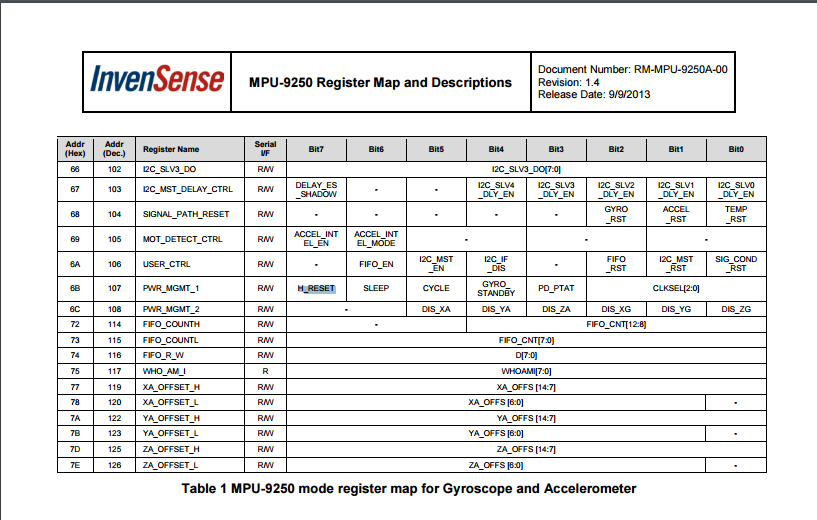
\includegraphics[width=0.5\textwidth]{images/reg.png}
\end{figure}

\subsubsection{Deep Neural Network}
Figure 5 illustrates the setup for training, exporting and importing a Tensorflow\cite{tensorflow} model directly into the CCS. This setup allows us the flexibility and speed of being able to train deep neural networks using the latest mechanisms on host CPUs+GPUs, and then moving weight matrices from trained models as 32-bit binary-float arrays, nicely wrapped here as a .model file. Source on GitHub provides clean/hassle-free C/python reading and writing utilities for .model files. In CCS, it is as simple as including "DNN.h", and calling DNNRead(), or DNNWrite().
\begin{figure}[h!]
  \caption{System Overview - Tensorflow + DSPLIB framework}
  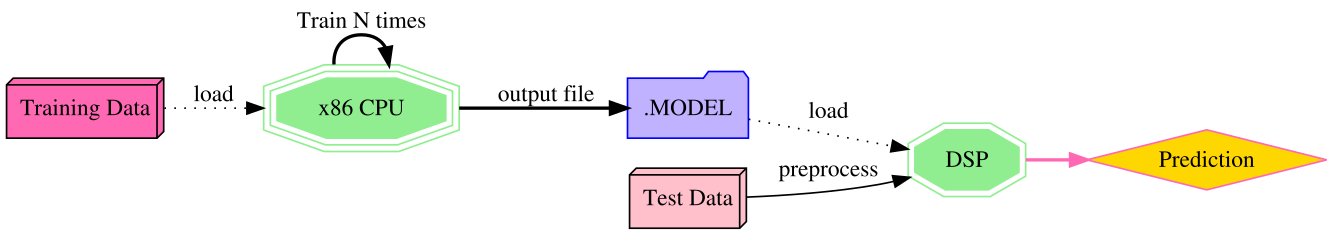
\includegraphics[width=0.5\textwidth]{images/train.png}
\end{figure}
On the LCDK side, DNNs are read into memory and input data is passed to the DNN using the function int DNNPredict(float *data), which returns an integer value for the predict class, or negative -1 if there is an internal error.

\subsection{Procedure - Plan and Implementation}
\subsubsection{Compute Performance}
We began optimization by using TI provided libraries DSPLIB, MATHLIB, and IMGLIB, and comparing their performance with the TI standard provided headers such as math.h and the infamous fft.h. We then wrote tests bench-marking multiple functions, with varying array sizes and operation-count. The figure below illustrates example usage for the profiler code.
\begin{figure}[h!]
  \caption{Example Profiler Code Usage}
  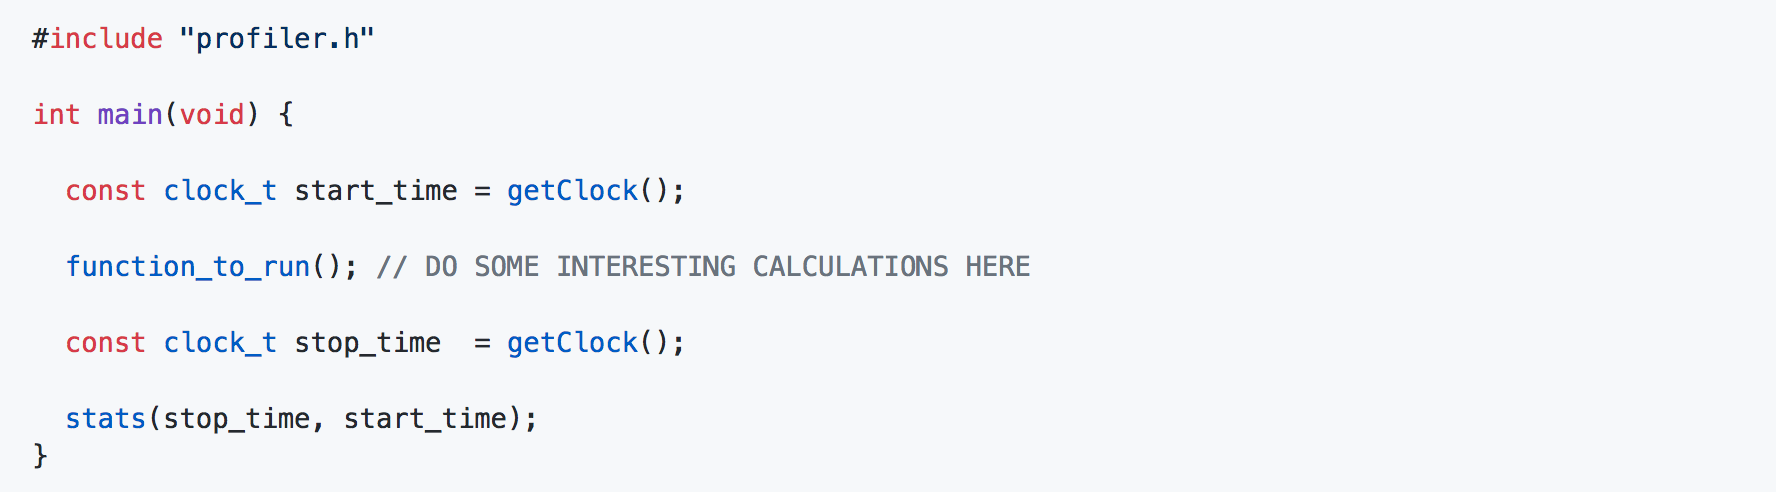
\includegraphics[width=0.45\textwidth]{images/profiler.png}
\end{figure}

\subsubsection{Communication Protocols}
On the LCDK, in order to enable any of the communication protocols, an interrupt service routine has to be set up with an interrupt mask, along with an interrupt handler for the given event. If the interrupt is going to occur on the communication bus, then the pin-mux has to be set as well. Although one could set up multiple interrupt masks for UART and I2C simultaneously, one of the interrupts will not fire due to the multiplexing limitation.\\
\\\textbf{I\textsuperscript{2}C with 9-DOF MPU-9250} \\
Using StartWare samples for the LCDK, we begin by reverse-engineering the I\textsuperscript{2}C example code, exhaustively isolating and understanding each dependency. Once we have a good handle on the code, we write simple subroutines to send data bytes to the MPU-9250 9-DOF over the I\textsuperscript{2}C bus. The 9-DOF is connected to pins 13 (SDA) and 15(SCL) on the J15 header expansion board.  The 9-DOF address is fixed at 0x69. Starting data acquisition from the 9-DOF requires setting up the pin-mux, appropriately covering the Interrupt Service Routine with Interrupt Masks, and enabling the I\textsuperscript{2}C controller on the desired data address. Once the bus is set, data is written to the 9-DOF registers over I\textsuperscript{2}C and an ACK signal is received over the bus.\\

\textbf{Long Distance I\textsuperscript{2}C}\\
Although I\textsuperscript{2}C implements clock stretching, bus errors are still fairly typical for transmission lines longer than $15cm$ (@400kHz). These bus errors are a direct consequence of clock skew caused due to bus capacitance and noise on the data channel. In order to mitigate these effects without sacrificing throughput, we propose the addition of six circuit components, which include four pull-up resistors and two TI I\textsuperscript{2}C P82B96 bus buffers. The figure below illustrates the setup, where "Long Cable" is replaced with twisted pairs from a CAT-5E Ethernet cable and "12V" is replaced with "3V3". Since all voltages are a standard 3.3V, all pull up resistors are chosen to be in the range of 1K-2.2K. SDA and SCL pins connected to the 'Main Enclosure' connect with the powered master device, whereas the ones connected to the 'Remote Enclose' connect to the remote slave. With this setup, we are able to receive error-free I\textsuperscript{2}C over $8m$, although the untested theoretical limit is calculated to be $100m$.\\
\begin{figure}[h!]
  \caption{P82B96 + twisted pair I\textsuperscript{2}C Bus Buffer}
  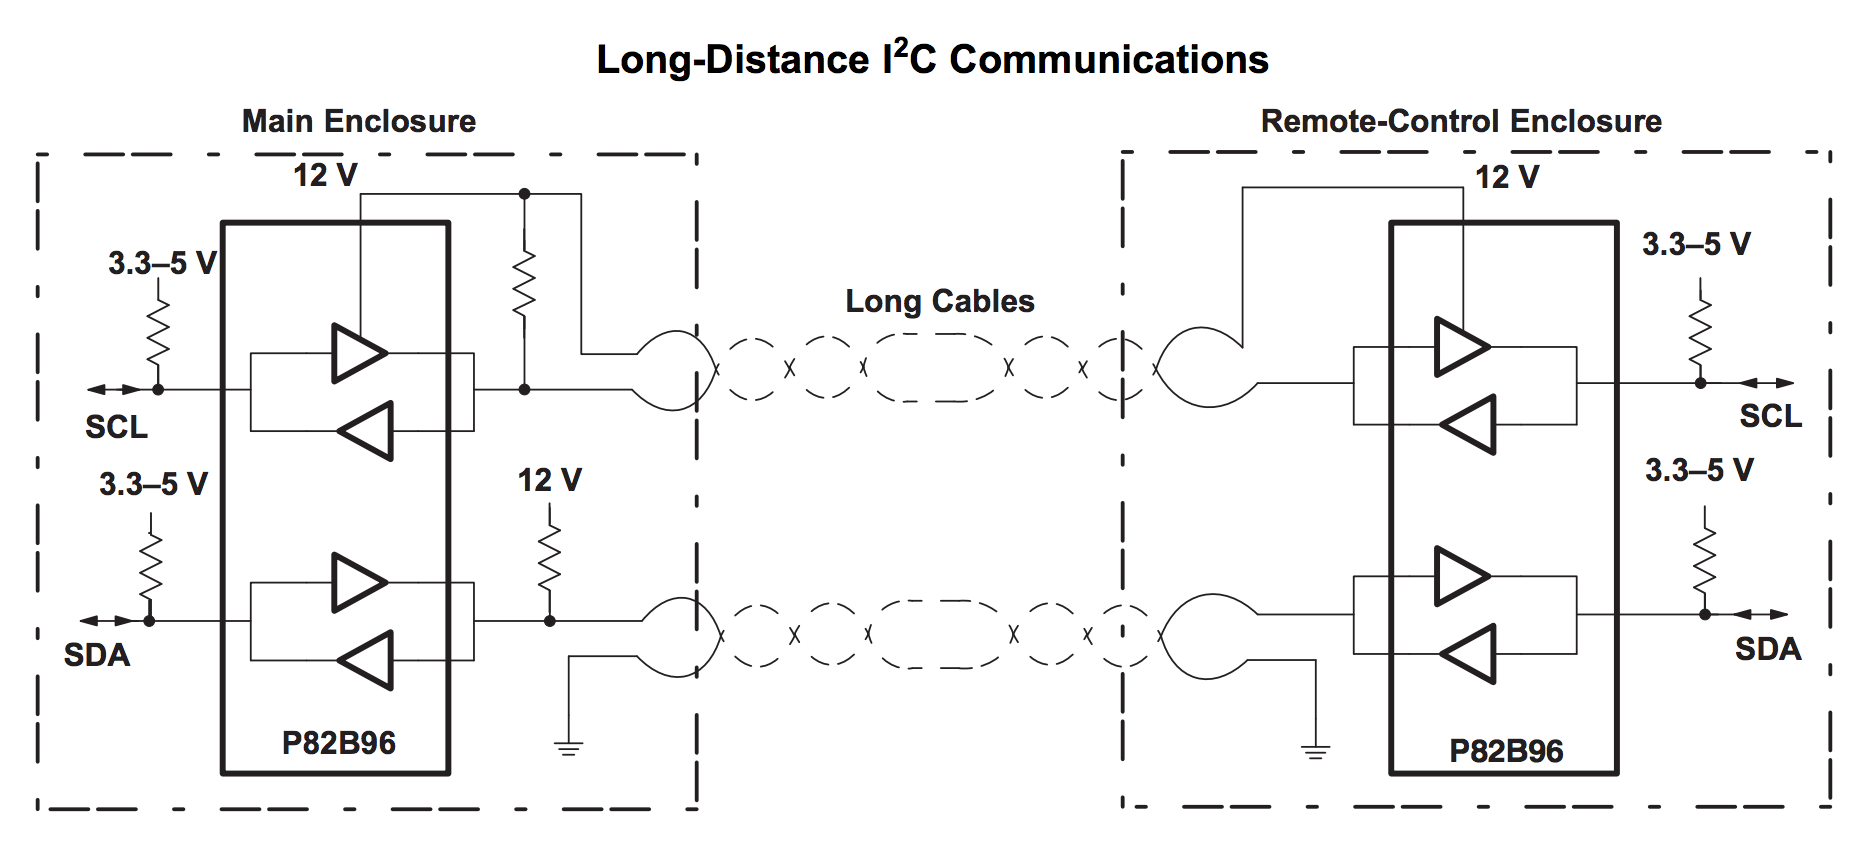
\includegraphics[width=0.5\textwidth]{images/buffer.png}
\end{figure}\\

\textbf{UART Protocol}\\
The LCDK hosts three UART controllers, one of which is used by the TI XDS100v2 emulator. We have been able to successfully use the other two. The first UART interface is exposed over USB-UART, and can be connected to through a USB-to-mini-USB cable. In CCS, once the pin-mux, interrupt service routines, and interrupt masks have been set, data can be sent and received at 115.2kbps baud rate over the UART port. The second UART port needs to be manually enabled by shorting out solder pads R206 and R209 on the back of the LCDK and connecting to pins 13 [RXD] and 15 [TXD] on the J15 expansion header.


\subsubsection{Deep Neural Network}
The following section documents the implementation and optimization process for matrix-backed neural networks on the LCDK.\\
% Activation Function
\\\textbf{Activation Functions} We begin by implementing an activation function. Of the various available options, $reLU(x)$ activations are known to be quite robust to input variance, and are efficient to implement. In interest of completeness, we also implement $tanh(x)$ and $sigmoid(x)$ functions, although these will not be used further, due to the additional need to normalize the inputs when using them and complex implementation. We then further optimize these functions using math ops from MATHLIB. The graph and equations below illustrate the these activation functions.
\begin{figure}[h!]
  \caption{Neuron Activation Functions}
  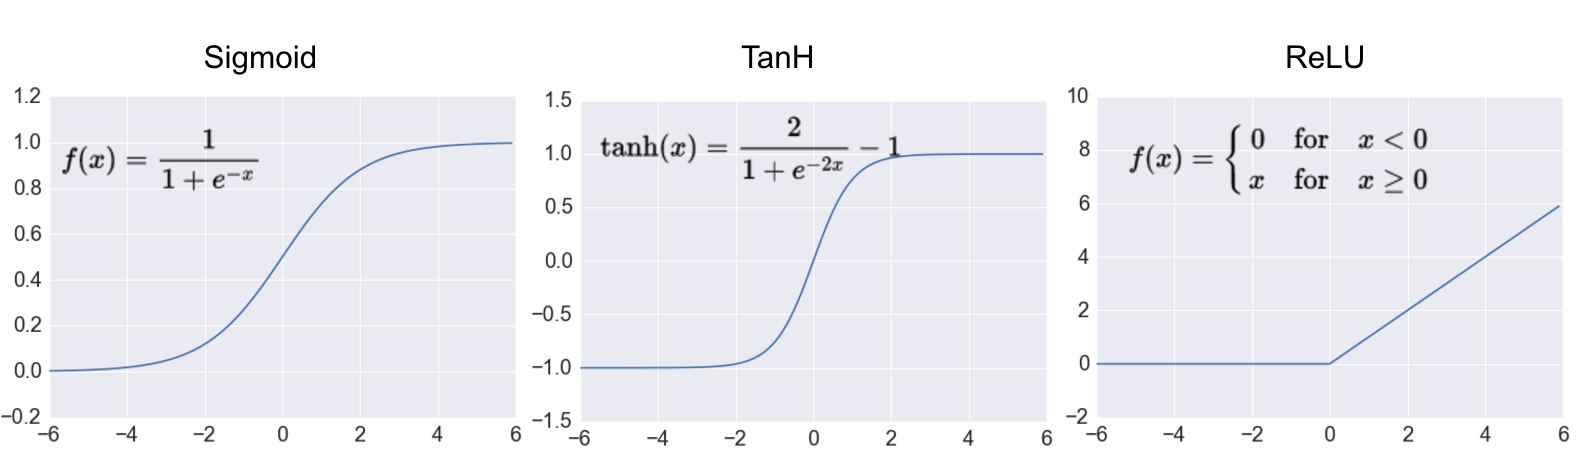
\includegraphics[width=0.5\textwidth]{images/activation.png}
\end{figure}
% Feed Forward
\\\textbf{Feed-forward step:} Next, we implement the matrix multiplications. Equation (1) depicts the matrix multiplication between the inputs and the first hidden layer. The weights of all hidden layers are stored in memory and are of the size $m*1*4$ bytes where $m$ is the number of features in the input. For all the cases below, $n=1$ since the batch-size is 1 (since we are making one inference at any moment in a real-time system).
\begin{figure}[h!]
  \caption{Weight Matrix Representation}
  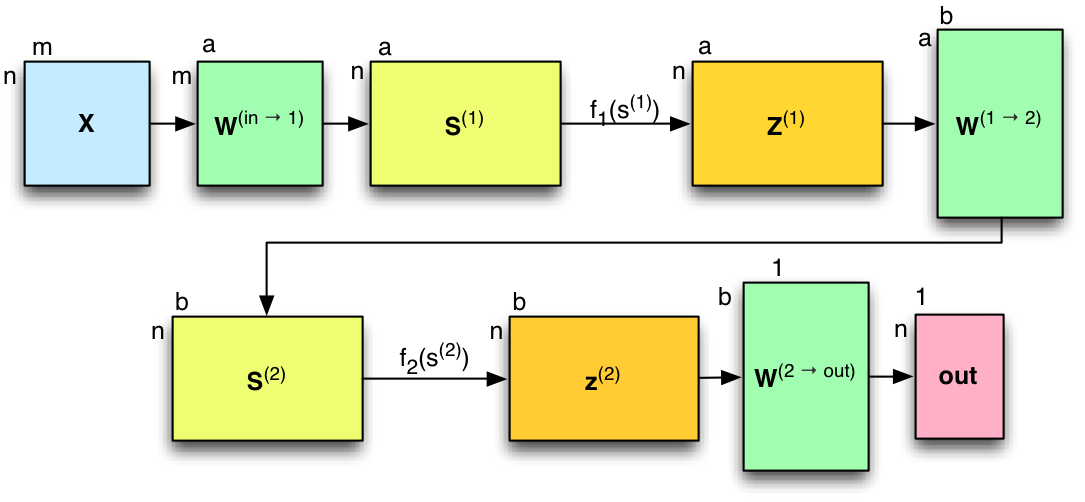
\includegraphics[width=0.5\textwidth]{images/matrix.png}
\end{figure}
\begin{align}
  S^{(1)} =&\ XW^{(in\rightarrow 1)}\\
  Z^{(1)} =&\ f_1(S^{(1)})\\
  S^{(2)} =&\ Z^{(1)}W^{(1\rightarrow 2)}\\
  Z^{(2)} =&\ f_2(S^{(2)})\\
  \hat{y} =&\ f_{out}\left(Z^{(2)}W^{(2\rightarrow out)}\right)
\end{align}

% Training
\textbf{Training in Tensorflow:} With the inference code implementation complete, we proceed to train our neural network in Tensorflow. We have pre-recorded accelerometer data (sampled every $62.5ms$) from a smartwatch. The data contains ambulation information. The table below illustrates some raw-data from the dataset.
\begin{center}
 \begin{tabular}{||c c c c||} 
 \hline
 accel_x & accel_y & accel_z & label \\
 \hline\hline
 8.707711 & 1.149216 & 1.879448 & walking \\
 \hline
 9.730036 & -0.694318 & 2.047042 & stationary \\
 \hline
\end{tabular}
\end{center}

After performing a training/testing split, the raw training data is fed into the neural network and trained using back-propagation\cite{backprop} with Adam\cite{adam} gradient descent. All source code has been made available on GitHub, along with tutorials to create new models. For reference, the table below illustrates the hyper-parameters tuned for our network. For a two second window, $32*3 = 96$ samples are recorded at 16samples/sec.

\begin{center}
\begin{tabular}{ c c }

Number of Inputs:  & 96 \\ 
Number of Outputs: & 2 \\ 
Hidden Layers: & {768, 384, 192, 96, 48, 24, 12, 6} \\ 
Learning Rate: & 0.005 \\  
L2 Regularization: & 0.001 \\
Batch Size: & 114 \\
Epochs: & 897  \\
\end{tabular}
\end{center}

Once the model has been built, it can be exported to the LCDK and mapped directly into memory using the CCS Memory Mapper utility. At this point, we enable our UART code, and read data from the slave device. The slave device is a Bluetooth controller, connected wireless to an Android device (smart-watch). Accelerometer data is streamed in real-time from the smart-watch directly into the input layers of the DNN on our LCDK.